% !TeX spellcheck = da_DK
\bruno{Dette kapitel skal måske hedde farvekamera og så ende ud i at vi har valgt at bruge kinect fordi det er let at arbejde med}
 \section{Microsoft Kinect}\label{kinect}
En Kinect er et Natural User Interface (NUI) udviklet til Microsoft's spillekonsol, Xbox.
Dens primære formål er at gøre det muligt at interagere med sin konsol vha. bevægelse og talte kommandoer.
Dog har den også mange andre anvendelsesområder, f.eks.:
%Den første version der udkom i november 2010~\cite{kinectWiki} er oprindeligt udviklet med henblik på at lokke nye typer brugere til Xbox med det argument at det via naturlig (og aktiv) bevægelse er sjovere og mere virkelighedstro at spille.
%
%I februar 2012 blev der lanceret en ny type Kinect, kaldet Kinect for Windows, der sammen med et Software Development Kit (SDK), der gør det muligt at udvikle både kommercielle og non-kommercielle applikationer til Kinect der kan køres på Windows platformen.
%Kort fortalt er Microsoft's Kinect mere end en input enhed gamere kan bruge for at gøre deres spiloplevelse mere virkelighedstro; af andre anvendelser kan f.eks. nævnes~\cite[s.~17]{kinectProgrammingGuide}:

\begin{itemize}
\item Optagelse af video i real-tid
\item Generere et dybde billede ved hjælp af kameraet og de to IR sensorer
\item Vurdering af omgivelserne ved hjælp af lyd
\end{itemize}

Oprindeligt eksisterede der kun en Kinect til XBox, men i februar 2012 blev der lanceret en ny type kaldet Kinect for Windows, der sammen med et Software Development Kit (SDK), gør det muligt at udvikle både kommercielle og ikke-kommercielle applikationer til Windows platformen.

I dette projekt skal Kinecten benyttes til at bestemme en autonom robots placering i ukendte omgivelser. 
Følgende afsnit giver en kort introduktion til Kinecten's egenskaber der skal danne grundlag for hvorfor Microsoft Kinect er valgt som løsningsmetode til lokaliseringsproblemet.\cite{kinectProgrammingGuide}

\subsection{Opbygning af Kinect}\label{kinect:komponenter}
I denne rapport er det versionen Kinect for Windows der fokuseres på, da den giver bedst kompatibilitet med PC samt det faktum at den er tilgængelig gennem universitetet.

%Dog kan det nævnes at forskellene mellem den og versionen til Xbox er meget små.
%Hardware mæssigt har Kinect for Windows den fordel at firmwaren indeholder en såkaldt Near Mode, hvilket gør det muligt at følge objekter indtil 40 cm fra enheden.
%Kinect for Xbox har ikke denne funktionalitet, og kan derfor kun følge objekter indtil 80 cm fra enheden, hvilket kan blive et problem i situationer hvor man ønsker at detektere små afstande via dybdebilleder.
%Kinect for Windows kan desuden også benyttes til kommercielle applikationer, hvor dens pendant er beregnet til hobbyister, generel udvikling og forskning~\cite[s.~16]{kinectProgrammingGuide}.
%
%For at Kinecten kan følge et objekt er Kinecten udstyret med et antal sensorer der nu vil blive beskrevet.

\begin{figure}
\centering
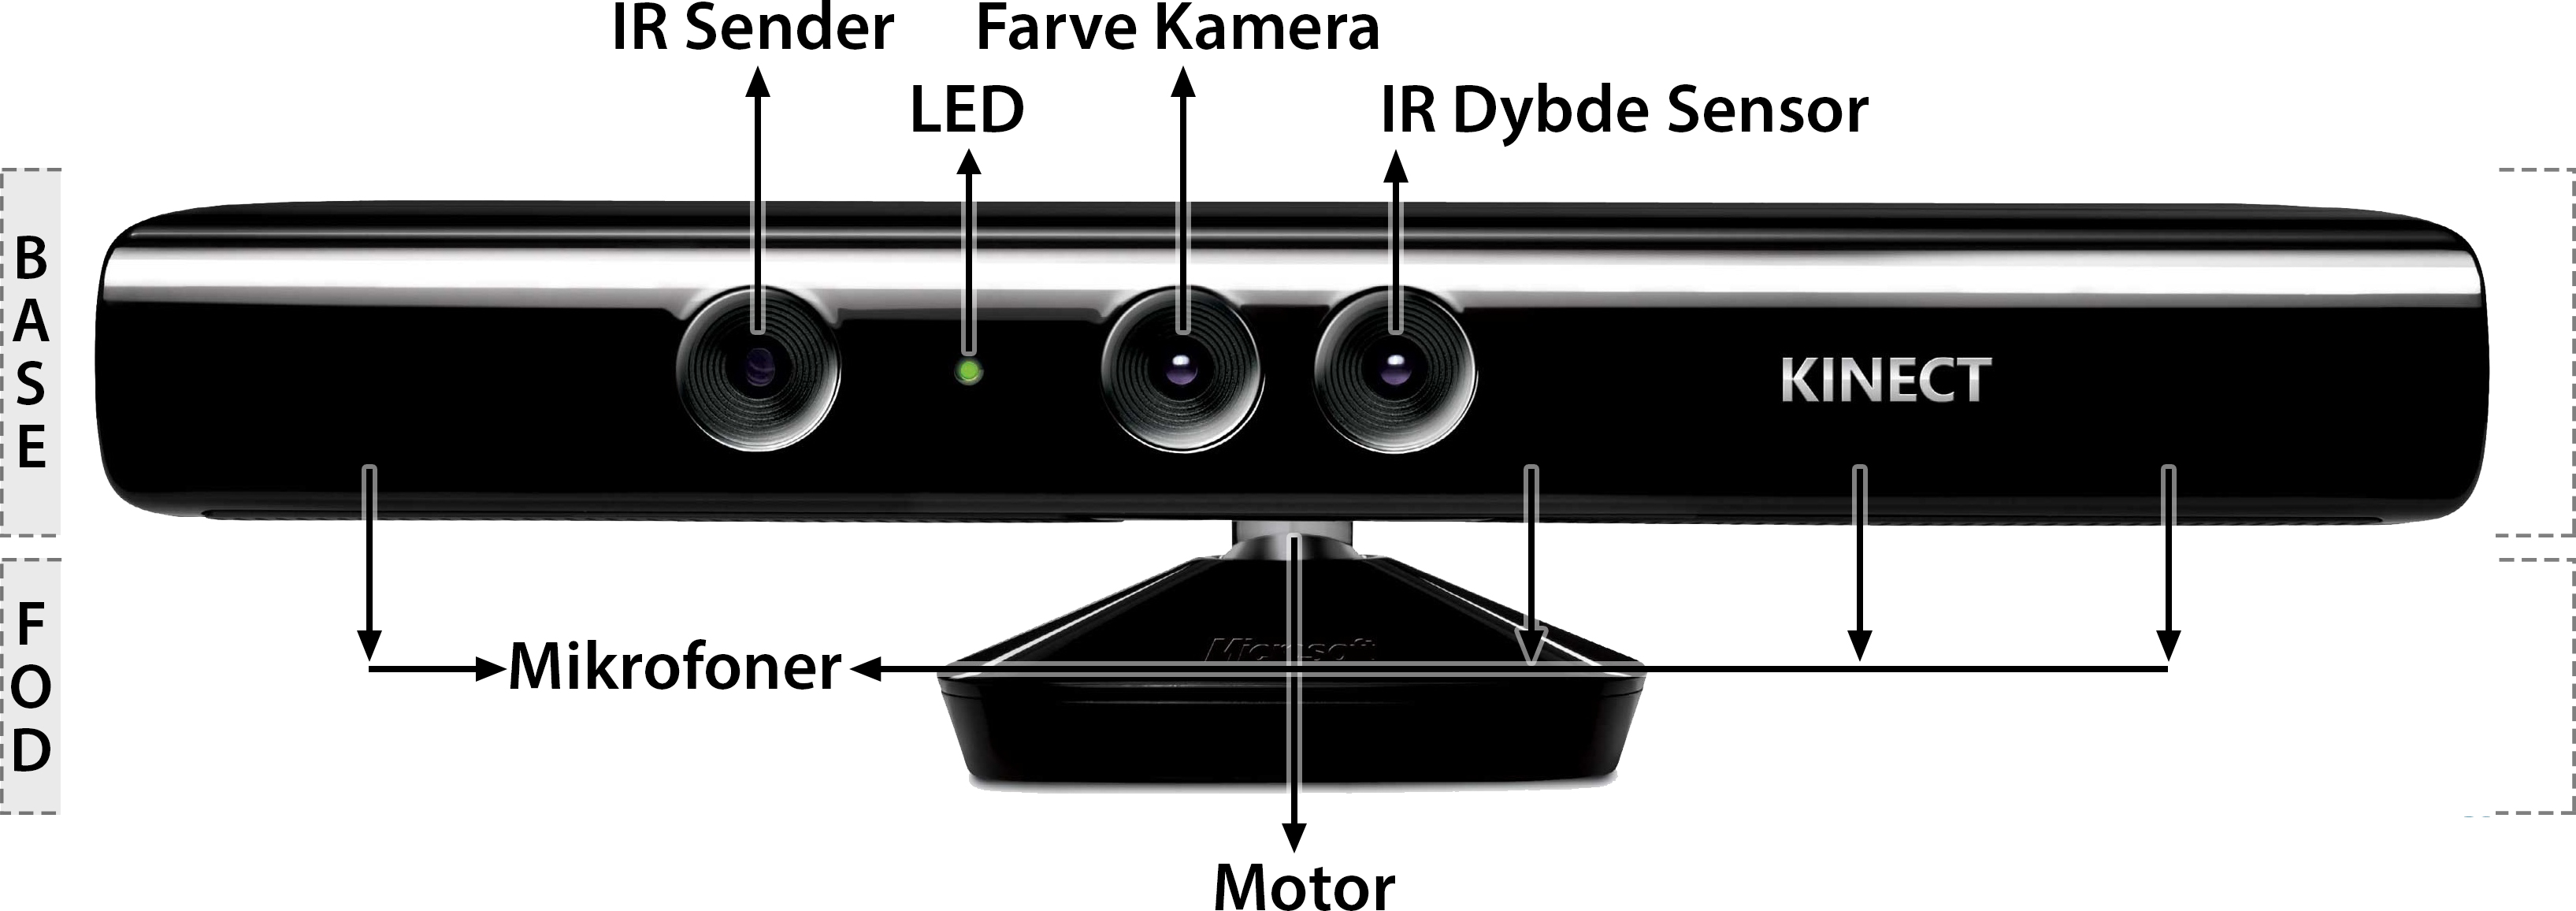
\includegraphics[width=1.0\textwidth]{kinect/kinect}
\caption{Microsoft Kinect for Windows}
\label{kinect:opbygning}
\end{figure}

Microsoft Kinect for Windows består af en mængde hardware som kan tilgås via det medfølgende SDK\footnote{Der findes også andre tredjeparts SDK'er til Microsoft Kinect, men som ikke er relevante ift. projektet, hvorfor de ikke nævnes.}.
Microsoft Kinect for Windows består af følgende komponenter:

\begin{itemize}
\item Farvekamera
\item Infrarød (IR) sender
\item IR dybde sensor
\item Mikrofoner
\item Motor til justering af vinklen
\item LED
\item Accelerometer
\end{itemize}

Microsoft Kinect for Windows kan ses på \cref{kinect:opbygning} sammen med dens synlige komponenter som står listed ovenover.

For at løse lokaliseringsproblemet er det valgt \textit{kun} at benytte Kinectens farvekamera, således der ses bort fra alle dens andre komponenter.
Derfor bliver farvekameraet på Kinecten i følgende afsnit beskrevet detaljeret ift. dets specifikationer.

\subsection{Farvekamera}\label{kinect:farvekamera}
For at gøre Kinecten i stand til at se, er den udstyret med et farvekamera som er placeret ca. i midten af enheden (jvf. \cref{kinect:opbygning}).
Videoen bliver sendt som en RGB videostrøm med mulighed for en opløsning på 1280x960 med en opdateringshastighed på 12 billeder i sekundet eller en lavere opløsning på 640x480 og 30 billeder i sekundet, hvis man ønsker en mere ”flydende” videostrøm~\cite{kinectForWindowsFeatures}.
Kinecten har en horisontal betragtningsvinkel på 57\degree~og en vertikal betragtningsvinkel på 43\degree, hvilket giver den et vertikalt synsfelt på $\pm 21.5$\degree, hvis den er placeret ift. 0\degree~vandret.
Et visuelt billede af Kinectens betragtningsvinkler kan ses på \cref{kinect:vinkler}.

\begin{figure}
\centering
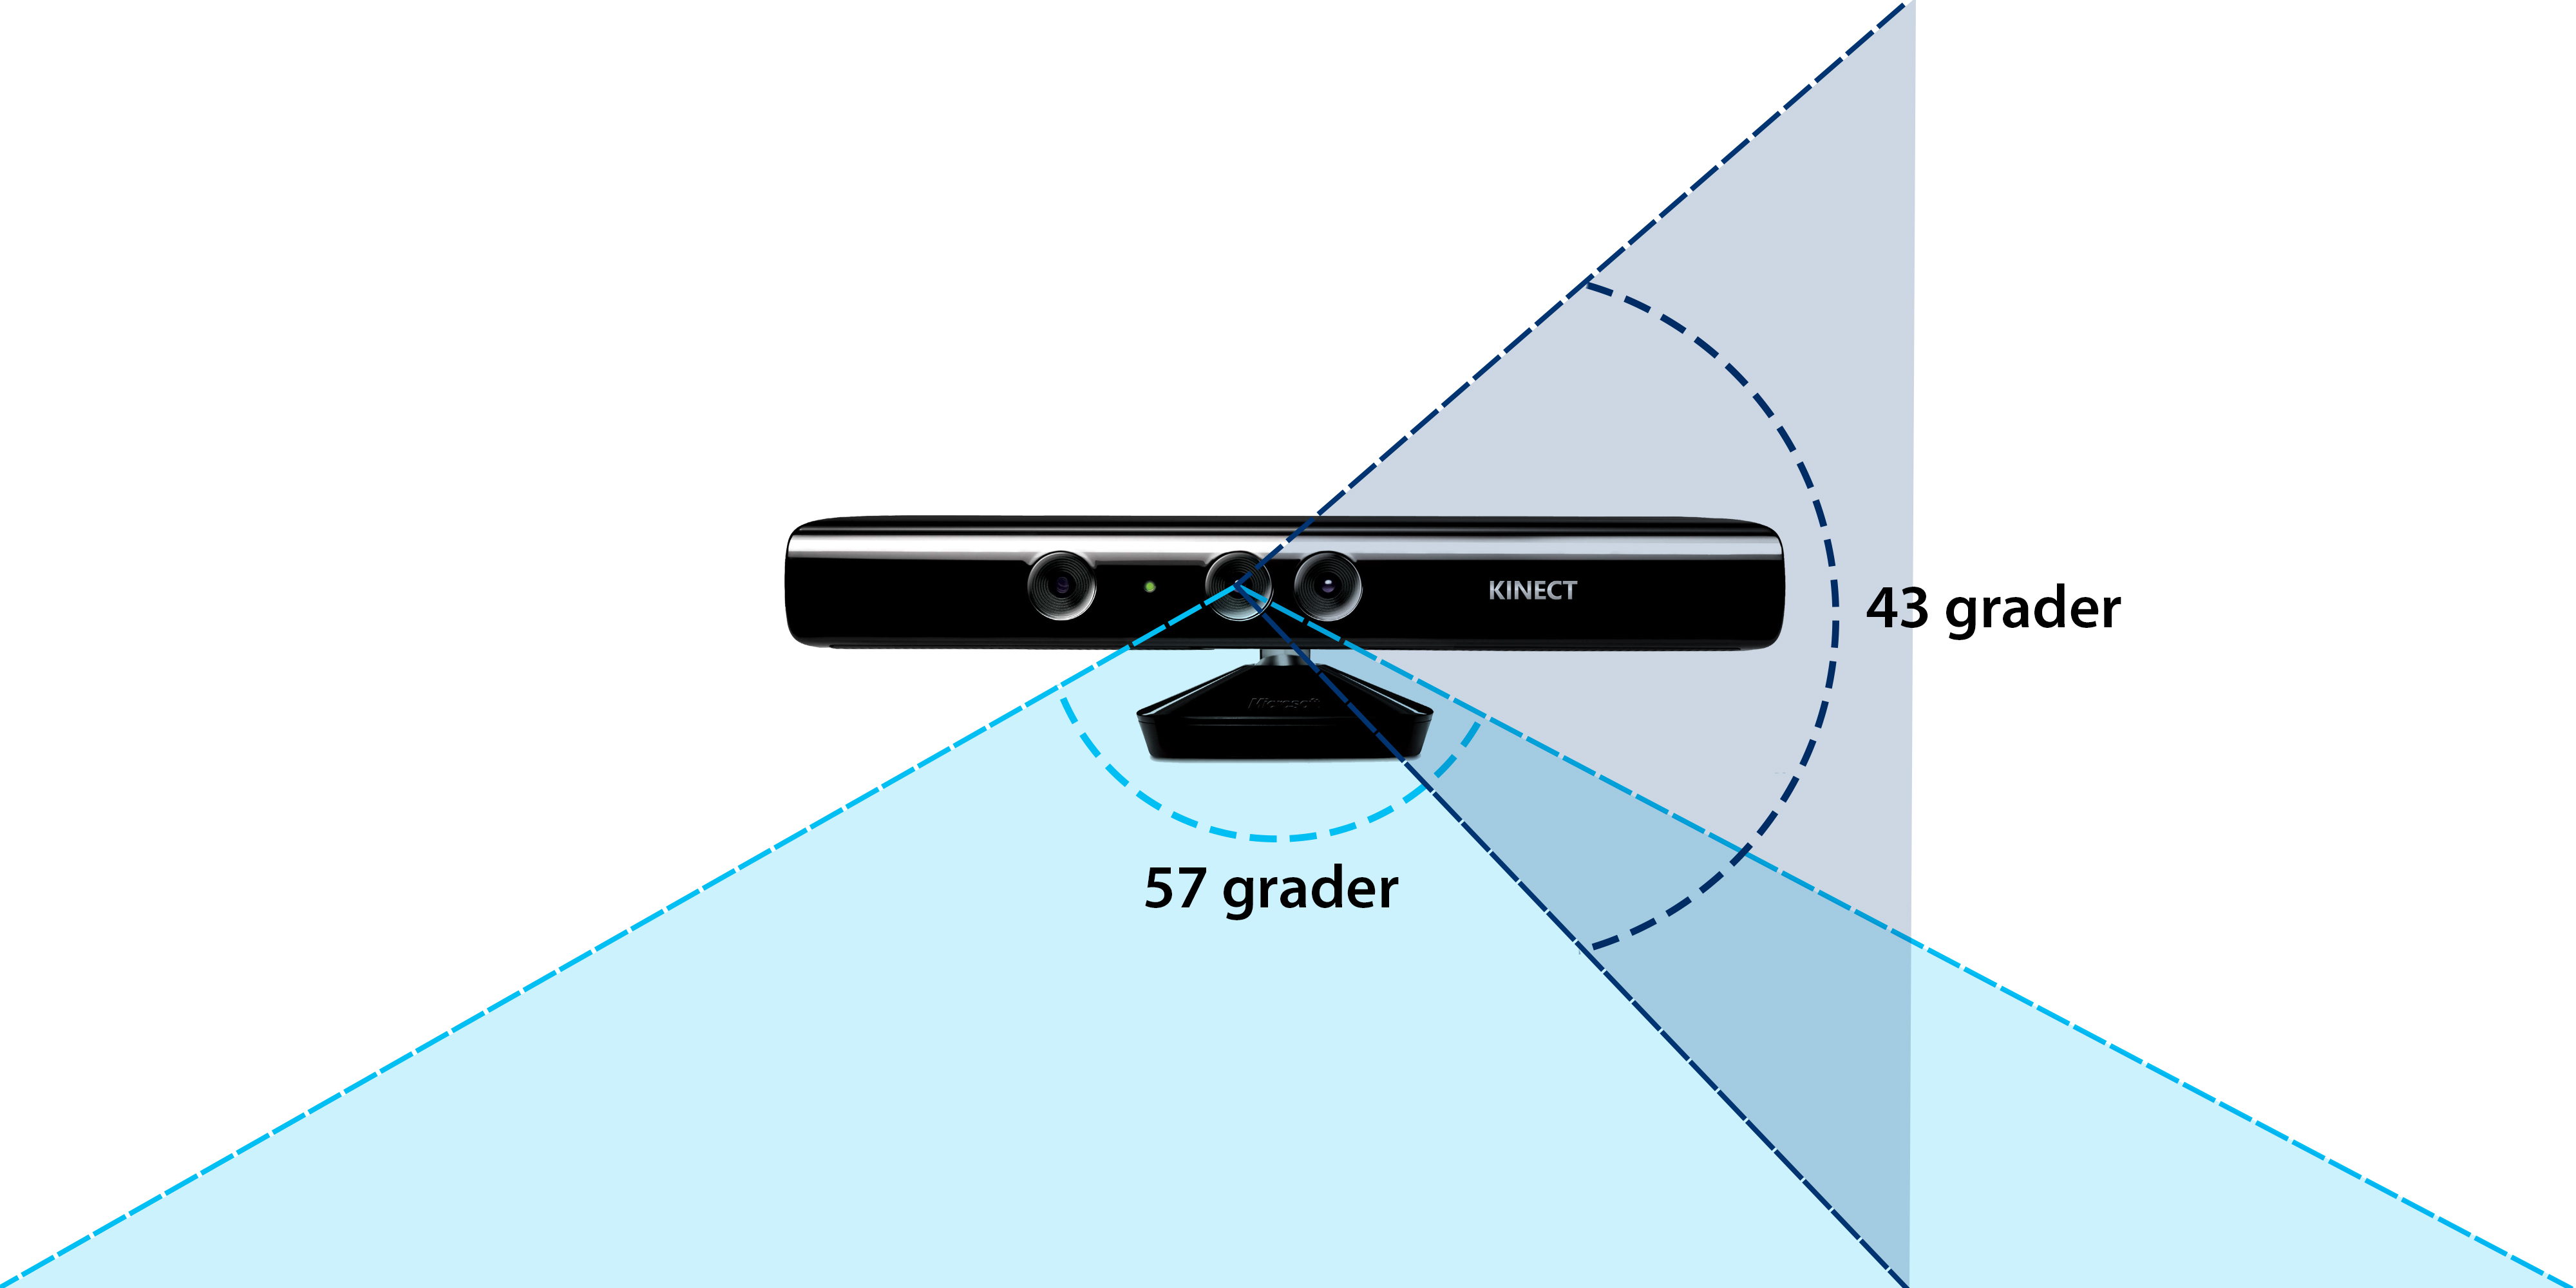
\includegraphics[width=1.0\textwidth]{kinect/kinect_view_angles}
\caption{Betragtningsvinkler for farvekameraet}
\label{kinect:vinkler}
\end{figure}

Disse parametre er interessante i forhold til hvilket formål der søges opfyldt med kinecten samt miljøet hvori den skal bruges. 
Det er f.eks. vigtigt at kende dens betragningsvinkler, hvis den skal benyttes til at lokalisere objekter med, da placeringer af disse skal placeres ift. deres fysiske placering, og ikke kun i Kinectens koordinatsæt.
Konverteringen mellem disse koordinatsæt er beskrevet yderligere i \cref{lokalisering:punktomregning}.

%\subsubsection{Infrarød (IR) sender}
%Metoden Kinecten benytter for at bestemme personers placeringer deres afstand fra Kinecten er vha. den infrarøde (IR) sender (\cref{kinect:opbygning}), som udsender et infrarødt lys der reflekteres så snart de rammer et objekt i rummet. 
%Disse signaler bliver fanget af en anden sensor på Kinecten; nemlig den infrarøde dybde sensor.
%
%\subsubsection{IR dybde sensor}
%Når det infrarøde lys bliver reflekteret tilbage mod Kinecten, bliver det opfanget af dybde sensoren (\cref{kinect:opbygning}), som konverterer lyset til dybde information, hvori man har en per-pixel afstand til de objekter der er tilstede i billedet.
%
%\subsubsection{Mikrofoner}
%Kinecten er også i stand til at optage lyd via de indbyggede mikrofoner.
%Dette er dog ikke det eneste mikrofonerne kan benyttes til; de kan også benyttes som en alternativ metode til at bestemme afstand og retning fra f.eks. en person der taler.
%Rækken af mikrofoner (se \cref{kinect:opbygning}) består af 4 stk. som er placeret på fronten af Kinecten.
%En enkelt mikrofon sidder i venstre side mens de tre andre er placeret til højre, hvilket gør det muligt at triangulere lydsignaler for at bestemme retningen af lydkilden.
%Flere mikrofoner gør det også muligt at lave ``noise-suppression'' ift. omgivelserne, hvis man benytter Kinect, mens man spiller, til at kommunikerer med sine med-/modspillere således at unødig støj filtreres fra~\cite[s.~15]{kinectProgrammingGuide}.
%
%\subsubsection{Motor til justering af vinklen}
%For at gøre det muligt for en Kinect at operere i flere forskellige miljøer og placeringer, er der indbygget en lille motor til at justere vinklen mellem Kinecten og foden den står på (jvf. \cref{kinect:opbygning}).
%Den kan bevæge sig fra 0\degree~til 27\degree~ (op) og fra 0\degree~til -27\degree~(ned).
%Denne funktionalitet er ideel hvis man ønsker at kalibrere Kinecten ift. dens fysiske placering og de omgivelser man ønsker at bruge den i.
%Dog anbefaler Microsoft at man ikke benytter motoren kontinuert i sine programmer, da den ikke tåler vedvarende belastninger~\cite{kinectDocElevationAngle}.
%
%\subsubsection{LED}
%Mellem kameraet og IR senderen er der placeret en status LED, der fortæller om driverne til Kinecten er indlæst korrekt eller ej.
%Dette kan være nyttigt for udviklere, da det giver sikkerhed for at kommunikationen mellem PC og Kinect er ok~\cite[s.~15]{kinectProgrammingGuide}.
%
%\subsubsection{Accelerometer}
%Kinect er også udstyret med et 3-akse accelerometer, som udvider den til andre anvendelsesområder end blot at følge (tracke) objekter og kropsbevægelser.
%Det er konfigureret til at give målinger fra -2g til 2g (mere præcis ved langsomme bevægelser end hurtige)~\cite{kinectAccelerometer}.
%Målingerne  er opbygget som en 3D vektor som peger mod tyngdekraften (gulv-planet), hvilket f.eks. gør det muligt at detektere om den er monteret korrekt (ovenpå eller under et fladskærms tv), således dens tilt kan korrigeres vha. den indbyggede motor.
%En anden interessant anvendelsesmulighed er at accelerometeret kan benyttes til at give bedre 3D projektioner i Augmented Reality.
%Ifølge dokumentationen~\cite{kinectDocAccelerometer}, er det præcist ned til en grad, dog med en nøjagtighed der kan varierer med op til 3 grader i forhold til rumtemperaturen.
%De skriver endvidere i dokumentationen at der kan kompensateres for denne unøjagtighed ved at sammenligne den vertikale måling (y-aksen i accelerometerets koordinatsystem) med den benyttede gulvplans dybdedata.

\subsection{Hvorfor Kinect}\label{kinect:argumentation}
Microsoft Kinect giver generelt mange muligheder pga. alle dens sensorer samt brugervenlighed overfor udviklere.
Dette har været vigtigt i forhold til at vælge at benytte en Kinect fremfor andre muligheder; f.eks. Nintendo's WiiMote eller et almindeligt webkamera.
At vælge en af disse andre muligheder opfattes af gruppen som en begrænsning, da det vil gøre det svært at ændre krav og tilpasse løsningen løbende, hvis dette skulle blive nødvendigt.
Derfor vil der fremadrettet udelukket fokuseres på at benytte en Microsoft Kinect til løsning af lokaliseringsproblemet.
For at opsummere, så ser gruppen Kinecten's overordnede fordele som:

\begin{itemize}
\item Nem montering
\item Nem tilslutning til PC
\item Mange sensorer
\item Gode udviklingsværktøjer
\item Tilgængelig gennem universitetet
\end{itemize}

%Senere i rapporten præsenteres testmiljøet som robotten skal navigere rundt i (\cref{testmiljo:opsaetning}).
%Den viste opsætning giver mulighed for at følge robotten fra en vertikal position ovenover testmiljøet, 

Ovenstående fordele giver mange muligheder i forhold til hvordan Kinecten kan benyttes, men da der stræbes efter en simpel og pålidelig metode vil dette smitte af på den endelige løsning.
Kinectens mange muligheder mht. tracking overvejes således ikke med mindre første løsning med kun at benytte farvekameraet ikke viser sig tilstrækkelig.

For at løse lokaliseringsproblemet ved blot at benytte et farvekamera vil der blive fokuseret på at genkende unikke farver i billedet, for derved at kunne udregne robottens lokation.
\thilemann{her mangler nok lidt mere argumentation/beskrivelse!}
Hvordan \textit{colortracking} er implementeret i praksis, står detaljeret beskrevet i \cref{tracking}.

\thilemann{Jeg kan ikke helt vurdere hvorvidt dele af dette afsnit er lidt en gentagelse af forrige afsnit, og om det i så fald gør noget?}

\section{Kinect for Windows SDK}
Til Kinecten findes der et officielt SDK\footnote{ Version 1.8, Udgivet 17 september, 2013~\cite{kinectSDK18}}, som åbner op for al funktionalitet i Kinecten med support fra Microsoft.

API'en er bygget op omkring en solid forståelse for menneskers bevægelser og karaktertræk således API'en kan fungere som et interface der kan genkende personers bevægelser, følge ansigter, genkende gestus og tale.
%Med Microsoft Kinect Toolkit installeret kan man endvidere få adgang til Kinect Fusion der gør det muligt at rekonstruere 3D objekter ud fra Kinectens kamera og dybdebilleder fra IR sensorerne.~\cite{kinectForWindowsFeatures}

\subsection{Kinect API}\label{kinect:kinectapi}
De følgende afsnit vil fokusere på hvordan SDK'et benyttes for at tilgå Kinectens mest basale funktionalitet med fokus på hvordan billeddata hentes fra dets farvekamera.

\subsubsection{Initialisering}
For at initialisere Kinecten og få adgang til dens sensorer skal Kinecten initialiseres.
Et eksempel på initialisering af en Kinect kan se på \cref{kinect:initialisering}. \lstinline[style=csharp]|Form1_Load| metoden i linje \ref{kinect:load} køres ved applikationens opstart og sørger for at starte sensoren hvis den findes. Fra linje \ref{kinect:enablebegin} til \ref{kinect:enableend} tændes for de billedstreams der er nødvendige. I eksemplet tændes for RGB-kameraet, dybdekameraet samt skeletdetektoren. Hvis der ikke er en Kinect tilsluttet meldes der fejl (linje \ref{kinect:error}).

\begin{lstlisting}[style=csharp, label=kinect:initialisering, caption={Initialisering af en Kinect sensor}]
KinectSensor sensor;

private void Window_Loaded(object sender,
	RoutedEventArgs e) (*\label{kinect:load}*)
{
    if (KinectSensor.KinectSensors.Count > 0)
    {
        this.sensor = KinectSensor.KinectSensors[0];
        StartSensors();
        
        this.sensor.ColorStream.Enable();(*\label{kinect:enablebegin}*)    
	this.sensor.DepthStream.Enable();
        this.sensor.SkeletonStream.Enable();(*\label{kinect:enableend}*)
	this.sensor.ColorFrameReady += 
		sensor_ColorFrameReady; (*\label{kinect:event}*)
    }

    else
    {
        MessageBox.Show("No Kinect connected"); (*\label{kinect:error}*)
        this.Close();
    }

}

private void StartSensors()
{
    if (this.sensor != null && !this.sensor.IsRunning)
    {
        this.sensor.Start();
    }
}
\end{lstlisting}

\subsubsection{Visning af Kinectens billeddata}
For at vise de billeder som Kinecten optager benyttes \lstinline[style=csharp]!sensor_ColorFrameReady! eventet. 
Dette event affyres hver gang der modtages et nyt billede fra Kinecten. 
Et eksempel på at vise Kinectens data ses på \cref{kinect:picture}, hvor der i linje \ref{kinect:openframe} gemmes en reference til den frame der netop er blevet optaget af Kinecten.
I linje \ref{kinect:pixeldata} kopieres data over i et bytearray for at arbejde på dataen. 
I linje \ref{kinect:source} sættes billedets source til et billede konstrueret ud fra dataen fra Kinecten.
Billedet \lstinline[style=csharp]|imageFrame| viser nu hvad Kinecten ser.

\begin{lstlisting}[style=csharp,caption={Visning af billeddata fra Kinectens RGB-kamera}, label=kinect:picture]
byte[] pixelData = null;
void sensor_ColorFrameReady(object sender,
	ColorImageFrameReadyEventArgs e)
{
    using (ColorImageFrame imageFrame = 
    	e.OpenColorImageFrame()) (*\label{kinect:openframe}*)
    {
        if (imageFrame == null)
            return;

            this.pixelData = 
            	new byte[imageFrame.PixelDataLength];(*\label{kinect:pixeldata}*)

            imageFrame.CopyPixelDataTo(this.pixelData);

            int stride = imageFrame.Width *
            	imageFrame.BytesPerPixel;

            this.KinectImage.Source = 
            	BitmapSource.Create(
            imageFrame.Width, imageFrame.Height, 
            	96, 96, PixelFormats.Bgr32, null, 
            		pixelData, stride); (*\label{kinect:source}*)
    }
}    
\end{lstlisting}